Comma-separated value (CSV) files store data, both numeric and text, as
plain text. Because of this, CSV files provide two main benefits: they
can be opened using a wide variety of software, including free and
open-source software, and they are not tied to any particular version of
software. This flexibility makes CSV files particularly well suited for
collaboration and for data sharing. For example, Dryad, the online data
repository for data underlying peer-reviewed publications, prefers the
use of plain-text formats such as CSV. As the use of such public
repositories is increasingly required by journals such as Evolution,
Molecular Ecology, and American Naturalist, developing a workflow using
CSV files can greatly facilitate the publishing process.

\section{Structure of CSV Files}

While there is no official structure to CSV files, there is a common
format often followed when dealing with data. In particular, data should
be organized as a table, with one record per row, and where each record
has the same number of elements. Each element in a record is delimited
with a specified \emph{delimiter}. Although the use of commas as
delimiters is common, as the name implies, other delimiters such as tabs
and semicolons are also frequently used. Each element can be text,
numeric data, or a combination of the two. For example, the following is
a valid CSV entry:

\begin{lstlisting}
Wild Type, 2, 3.0, 8/2
\end{lstlisting}

This example has four elements per entry. The first element, \emph{Wild
Type}, is text. The second and third elements are numeric data. Finally
the fourth element contains a combination of numeric and text data.
Whenever text data are included, that element is interpreted as text.

Because CSV files arrange data in a tabular format, each element shares
some relationship with the corresponding element in other records. In
other words, the elements along each column should contain data
corresponding to the same aspect of whatever is being recorded in the
dataset. In the example data above, the first element in each record
represents the phenotype of the organism for which the measurement was
taken.

\subsection{Annotating CSV Files}

To make datasets easier to understand, \emph{metadata}, or additional
information about the data, can be added through the use of
\emph{headers} and \emph{comments}. A header row is used to describe the
data stored in each column of a dataset. Although there is no official
specification, many software packages that support headers expect them
to be on the first line of the file.

Comments allow CSV files to contain additional notes about the data,
such as a description of when and where the data were acquired, how the
dataset was obtained, or any remarks about a specific data point.
Comments are identified by a single character, typically \lstinline!#!,
at the beginning of a line, and specify that all subsequent text on that
line should be ignored. For comments that span multiple lines, a comment
character must be included at the beginning of each line. The following
dataset includes both headers and comments:

\begin{lstlisting}
Temperature,Row,Column,Luminescence
# Luminescence of evolved V. harveyi
# Eric Bruger - 2012/06/27

26.3,0,0,7444.945
26.3,0,1,4845.375
26.3,0,2,4056.362
# Look at this luminescence!!!
26.3,0,3,4883.137
26.3,0,4,3593.289
26.3,0,5,2645.281
26.3,1,2,10507.588
\end{lstlisting}
It is important to note, however, that not all programs that support
CSV-formatted files support headers or comments. When using these
programs, these metadata should first be stripped from the file. This
can easily be done with several common tools available on the Unix
command line, which will be introduced later in this chapter.
Alternately, thee metadata can be removed manually or with a script.

\subsection{Including Replicates}

In most cases, data sets will contain measurements from multiple
replicates. For example, the luminescence data might contain data from
reads of multiple plates. Since these data describe the same thing, it
makes sense for them to be stored in the same file. However, if we just
added these data to the end of file, it would not be possible to
differentiate between the data for row 0, column 0 of the one plate and
any other plate if we keep with the Temperature-Row-Column-Luminescence
format.

To handle replicates, we can add a new column for each entry that
specifies the plate from which each data point were acquired.

\begin{lstlisting}
Plate,Temperature,Row,Column,Luminescence
# Luminescence of evolved V. harveyi
# Eric Bruger - 2012/06/27

Plate1,26.3,0,0,7444.945
Plate1,26.3,0,1,4845.375
Plate1,26.3,0,2,4056.362
Plate1,26.3,0,3,4883.137
Plate1,26.3,0,4,3593.289
Plate1,26.3,0,5,2645.281
Plate2,30.0,0,0,5713.744
Plate2,30.0,0,1,3491.94
Plate2,30.0,0,2,2851.252
Plate2,30.0,0,3,3872.232
Plate2,30.0,0,4,2632.069
Plate2,30.0,0,5,1594.228
\end{lstlisting}
\subsection{Time Series Data}

Similarly, time series can be thought of as measurements replicated over
time. To augment our data set to show multiple reads of the plates over
time, we can simply add a column that indicates when the measurement was
taken:

\begin{lstlisting}
Plate,Time,Temperature,Row,Column,Luminescence
# Luminescence of evolved V. harveyi
# Eric Bruger - 2012/06/27

Plate1,0:00,26.3,0,0,7444.945
Plate1,0:00,26.3,0,1,4845.375
Plate1,15:00,30.1,0,0,6088.0
Plate1,15:00,30.1,0,1,3976.694
Plate1,30:00,30.0,0,0,6563.678
Plate1,30:00,30.0,0,1,4188.048
Plate2,0:00,30.0,0,0,6716.929
Plate2,0:00,30.0,0,1,4153.633
Plate2,15:00,30.0,0,0,6672.662
Plate2,15:00,30.0,0,1,4167.991
Plate2,30:00,30.0,0,0,5810.844
Plate2,30:00,30.0,0,1,3652.258
\end{lstlisting}
As another example, the data below show reaction counts in one Avida
population over 1,000 updates for one population:

\begin{lstlisting}
Update,NOT,NAND,AND,ORN,OR,ANDN,NOR,XOR,EQU
# Reaction counts
# Brian Connelly - 2012/03/03

98000.0,172.0,2.0,33.0,35.0,2167.0,1007.0,4377.0,0.0,0.0
98100.0,195.0,4.0,40.0,28.0,2185.0,1085.0,4408.0,0.0,0.0
98200.0,191.0,2.0,37.0,31.0,2147.0,1004.0,4278.0,0.0,0.0
98300.0,177.0,5.0,32.0,27.0,2239.0,904.0,4363.0,0.0,0.0
98400.0,191.0,6.0,45.0,30.0,2285.0,986.0,4390.0,0.0,0.0
98500.0,187.0,11.0,34.0,22.0,2277.0,1072.0,4485.0,0.0,0.0
98600.0,205.0,6.0,38.0,38.0,2417.0,956.0,4449.0,0.0,0.0
98700.0,158.0,7.0,48.0,21.0,2461.0,930.0,4501.0,0.0,0.0
98800.0,176.0,8.0,58.0,20.0,2265.0,931.0,4267.0,0.0,0.0
98900.0,150.0,5.0,45.0,31.0,2199.0,1030.0,4440.0,0.0,0.0
\end{lstlisting}
Avida output data can be converted to CSV using the
\lstinline!avida2csv.py! script included with BEACONToolkit.

\section{Excel and CSV files}

Support for reading and writing data in CSV format is included in
Microsoft Excel and each of the Excel-like spreadsheet programs (e.g.,
Numbers, Google Docs, OpenOffice Calc). Like with the native formats,
CSV files can be opened with the \textbf{Open} item in the \textbf{File}
menu.

To save data as a CSV file in Excel, the \textbf{Save As} item in the
\textbf{File} menu is used. Shown below, the \emph{Format} should be set
to \emph{Comma Separated Values (.csv)}. Menu options for other
spreadsheets vary slightly.

\begin{figure}[htbp]
\centering
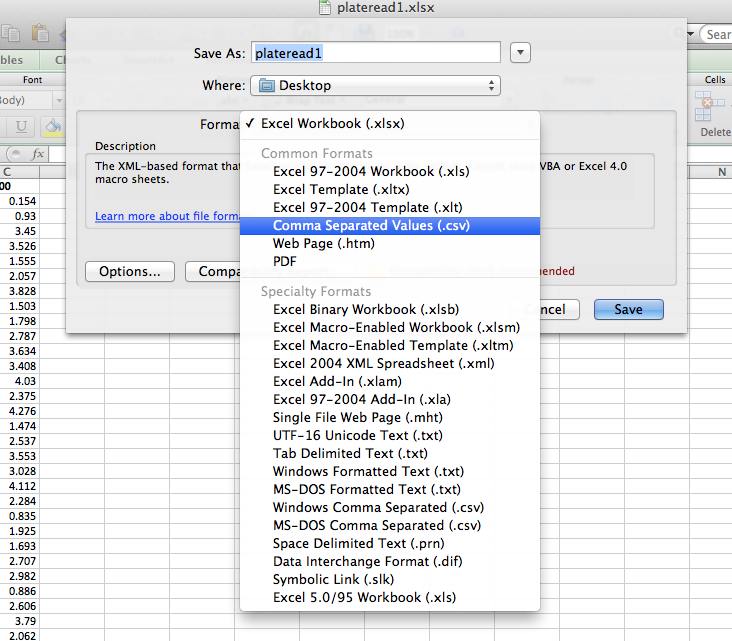
\includegraphics[width=0.80\columnwidth]{../csv/doc/figures/excel-saveas.png}
\caption{Saving data as CSV with Excel}
\end{figure}

It should be noted, though, that formulas included in spreadsheets will
not be saved in the resulting CSV files, only their values.

\subsection{Transposing Column-Based Data}

CSV data is intended to be row-based, with each row representing a data
point. To export data that have been arranged in a column-based layout
(see example below), the data must first be transposed.

\begin{figure}[htbp]
\centering
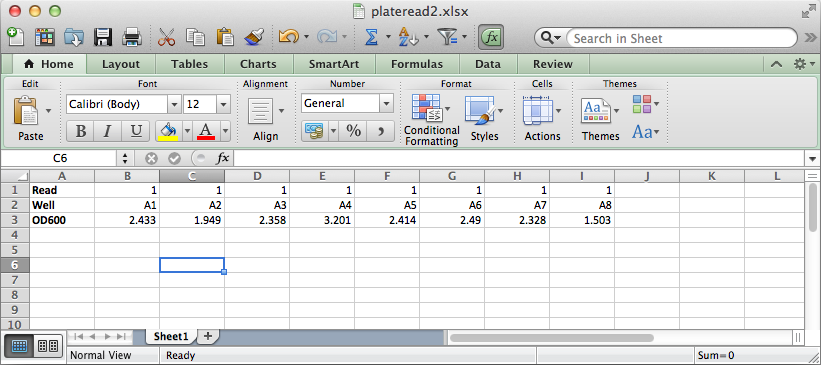
\includegraphics[width=0.80\columnwidth]{../csv/doc/figures/excel-horizdata.png}
\caption{Column-based data in Excel}
\end{figure}

The easiest way to accomplish this is to select the data and copy it.
Then, select the cell that will be at the upper left area of the
transpose data, select \textbf{Paste Special\ldots{}} from the
\textbf{Edit} menu, and choose the \emph{Transpose} option before
selecting the \textbf{OK} button.

\begin{figure}[htbp]
\centering
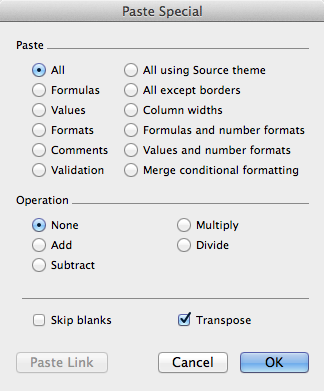
\includegraphics[width=0.50\columnwidth]{../csv/doc/figures/excel-paste_special.png}
\caption{Excel's \textit{Paste Special} Dialog Window}
\end{figure}

Now that the data are arranged in rows, the other data can be deleted,
and the spreadsheet can be saved as a CSV file as described previously.
This method of copying data and pasting transposed is only supported in
Excel and OpenOffice Calc.

In Google Docs (as well as Excel), data can be transposed using the
\textbf{TRANSPOSE} function. To do this, first select a region of empty
cells that is equal in size to the data to be transposed. For example,
if the column-based data occupies 3 rows by 9 columns as in the picture
above, select an area that is 9 rows by 3 columns. Once the target
region has been selected, enter:

\begin{lstlisting}
=TRANSPOSE(A1:I3)
\end{lstlisting}
To take the data from the region bounded by cells A1 in the upper left
and I3 in the lower right, transpose it, and paste it into the selected
region. Excel users should conclude entering this formula with
Control-Shift-Enter instead of Enter.

Unfortunately, Numbers does not provide any easy ways to transpose data.
The best plan for these situations would be to export the column-based
data as a CSV file, read that file using the Python tools described
later in this Chapter, and transpose the data in Python with a function
like \emph{transpose} in NumPy.

\section{R and CSV files}

Excel is a great tool for creating CSV files and for doing quick
analyses, but often using another tool built specifically for data
manipulation and analysis will prove useful. Using R (or Python) for
your data needs has many advantages including the ability to save
analysis scripts so they can be applied to new or different datasets
easily, and a large open-source community constantly contributing new
packages. The R language is particularly well suited for data anlysis
since it was originally written by statisticians, and they still make up
a large userbase.

\subsection{Reading CSV files}

Since data is so central to R, dealing with CSV files is remarkably well
incorporated into to the language's base functionality. The most common
way to read CSVs, and the one we will use here is \lstinline!read.csv!.
You can see the R help page for this function by typing
\lstinline!?read.csv! as well as some information about other functions
you can use to import data.

First, we should tell R which directory we'll be working in so it knows
where to load files from. We can do that with the \lstinline!setwd!
function:

\begin{lstlisting}[language=R]
setwd('~/BEACONToolkit/csv/data')
\end{lstlisting}
Don't worry too much about the \lstinline!~/! in the path, it is a Unix
way of addressing relative directories. If you're using Windows, you may
run into a few gotchas with directories. The easiest way to get around
all of them is to always use full paths (i.e., ignoring the
\lstinline!~/!) and always forward slashes instead of backslashes. For
example, if your data was located in
\lstinline!C:\MyFiles\BEACONToolkit\csv\data! you should instead type:

\begin{lstlisting}[language=R]
setwd('C:/MyFiles/BEACONToolkit/csv/data')
\end{lstlisting}
Now that we have set R's working directory, we can ask R what files are
in there using the \lstinline!list.files! function. R is not meant to be
a repleacement for the terminal or file browser, but this quick way of
viewing the contects of a directory is helpful when you forget the exact
name of the file you want to load. If we run this function with our
working directory set to the \lstinline!BEACONToolkit/csv/data!
directory, we should see our two example datasets:

\begin{lstlisting}[language=R]
list.files()

# output
[1] "avida_reactions.csv" "luminescence.csv" 
\end{lstlisting}
We can now import this data using the \lstinline!read.csv! function.
Calling this function will return a \lstinline!data.frame! object, which
is R's way of internally representing tabular data. We want to store
this dataframe in a variable so we can use it over and over without
having to load the data every time. To do this in R, we simply run the
following command:

\begin{lstlisting}[language=R]
lum_data <- read.csv('luminescence.csv')
\end{lstlisting}
But if we take a look at this data, we can see there is a problem. The
\lstinline!head! function will list the first few rows of a dataset, and
is often usful to always run just to make sure there were no problems
importing the data. Running \lstinline!summary! will give you some
statistical summaries of the data, which is good for making sure the min
and max values of your data make sense, and to see if there are any
missing values. We can run these two functions, passing lum\_data as a
parameter (i.e., \lstinline!head(lum_data)! or
\lstinline!summary(lum_data)!). Another way of looking at the data is
using the \lstinline!edit! function. We will talk more about this
function in the Writing CSV files section.

\begin{lstlisting}
head(lum_data)

# output
                                 Plate        Time Temperature Row Column Luminescence
1 # Luminescence of evolved V. harveyi                      NA  NA     NA           NA
2           # Eric Bruger - 2012/06/27                      NA  NA     NA           NA
3                               Plate1 00:00:00:00        26.3   0      0     7444.945
4                               Plate1 00:00:00:00        26.3   0      1     4845.375
5                               Plate1 00:00:00:00        26.3   0      2     4056.362
6                               Plate1 00:00:00:00        26.3   0      3     4883.137
\end{lstlisting}
It looks like R thinks the comments are actually entries, and tried to
fit them into the dataframe. R does support comments in CSV files, but
by default the \lstinline!read.csv! function isn't expecting them.
Instead, we can be a little more explicit with our call to
\lstinline!read.csv!:

\begin{lstlisting}[language=R]
lum_data <- read.csv('luminescence.csv', header=TRUE, sep=',', comment.char='#')
\end{lstlisting}
The \lstinline!header! and \lstinline!sep! parameters, which let you
specify if the data contains a header row and the delimiter using to
seperate entries, are working correctly by default, but now you see how
easily they can be modified. Now if we take a look at our data, it is
correctly being imported by R.

\begin{lstlisting}
head(lum_data)

# output
   Plate        Time Temperature Row Column Luminescence
1 Plate1 00:00:00:00        26.3   0      0     7444.945
2 Plate1 00:00:00:00        26.3   0      1     4845.375
3 Plate1 00:00:00:00        26.3   0      2     4056.362
4 Plate1 00:00:00:00        26.3   0      3     4883.137
5 Plate1 00:00:00:00        26.3   0      4     3593.289
6 Plate1 00:00:00:00        26.3   0      5     2645.281
\end{lstlisting}
\subsection{Data Subsets and Selection}

Now that we have our dataframe, we can start pulling out data and
manipulating it using R. The simplest way to access data is by pulling
out an entire column. In R, we can access particular columns using the
\lstinline!$! operator, which extracts data from objects. To pull out
the Luminescence column from our dataset, we simply run:

\begin{lstlisting}[language=R]
lum_data$Luminescence
\end{lstlisting}
Another way we can access data is by indexing into the dataframe, which
is the same as indexing into a matrix in R. That means we can pull out
particular rows or columns using the \lstinline!data.frame[row,column]!
notation. For example, to pull out the Luminescence column (column 6) we
could also run:

\begin{lstlisting}[language=R]
lum_data[,6]
\end{lstlisting}
Leaving the \lstinline!row! spot blank tells R to return all of the rows
from column 6. We could also ask for particular rows instead of columns
by specifying the \lstinline!row! but not the \lstinline!column!, and
even ask for a single value by specifying both. R also lets you pass
vectors into the indecies. For example, maybe we wanted both Time and
Luminescence (columns 2 and 6) but didn't care about the rest. We could
run the following function, which would return a new
\lstinline!data.frame! object with only Time and Luminescence as
columns:

\begin{lstlisting}[language=R]
lum_data[, c(2,6)]
\end{lstlisting}
The \lstinline!c! function is short for \emph{combine}, which just
creates a vector out of the passed in values. Allowing vectors as
indexing arguments is very powerful and lets us use indexing as a way to
subset the data more flexibly. Perhaps we were only interested in the
data where Luminescence was at least 500,000 units. By asking R to only
return columns that meet the criteria
\lstinline!lum_data$Luminescence >= 500000!, we can get a new dataframe
containing a subset of our original data. Under the hood, this is
actually creating a \emph{masking vector} where each position is either
TRUE if Luminescence is greater than 500,000 or FALSE otherwise, and
then returns only rows corrosponding to TRUE values.

\begin{lstlisting}[language=R]
lum_data[lum_data$Luminescence >= 500000, ]
\end{lstlisting}
If we were only interested in particularly luminous data points from the
first row, we can add another logic statement to further subset the
dataframe:

\begin{lstlisting}[language=R]
lum_data[lum_data$Luminescence >= 500000 & lum_data$Row == 1, ] 
\end{lstlisting}
\subsection{Writing CSV files}

Because most of R revolves around \lstinline!data.frame! objects, it is
very simple to write new CSV files. Often it will be useful to
programmatically add columns or rows to data, and doing so with an R
script lets you easily re-create your changes should they be lost, apply
them to future data sets, as well as have a record of exactly how you
changed your data.

\section{Python and CSV files}

This section introduces three ways in which CSV files are commonly read,
manipulated, and written using Python. The first is Python's
\lstinline!csv! module, which is included in all Python installations.
The NumPy project, which provides a large collection of objects and
functions for scientific computing, also includes functionality for
working with CSV files. Finally, we introduce the CSV capabilities of
Pandas, a package aimed at providing tools for data analysis in Python.

\subsection{Python's csv Module}

Python's \lstinline!csv! module provides a number of objects that can be
used to read and write CSV files. Although these objects are generally
more bare bones than those described later in this section, they still
make working with CSV files in Python quite easy.

\subsubsection{Reading}

First, the following Python code opens and reads a CSV file named
\lstinline!luminescence.csv!:

\begin{lstlisting}[language=Python]
import csv

myreader = csv.reader(open('luminescence.csv', 'r'))
\end{lstlisting}
where \lstinline!'r'! specifies that the file will be opened for
reading. With this new object called \lstinline!myreader!, we can now
iterate through the contents of the CSV file line-by-line:

\begin{lstlisting}[language=Python]
for row in myreader:
    print "Read a row:", row
\end{lstlisting}
For each iteration of this loop, the \lstinline!row! variable contains a
list of values from that row. Because Python's list indices are
zero-based, the value in the second column of the current row is
accessed as \lstinline!row[1]!. This csv reader provides no
functionality for dealing with headers, comments, or empty lines, so
each \lstinline!row! may contain header information, comments, data, or
nothing. These shortcomings can be compensated for with additional code
to check the beginning of the file and to look for the presence of the
comment character.

Python reads each row as a collection of strings. To convert a value to
a numeric value, the \lstinline!int! and \lstinline!float! functions can
be used:

\begin{lstlisting}[language=Python]
for row in myreader:
    as_pct = float(row[2])/100
\end{lstlisting}
As a precaution, \lstinline!int! should only be used when your are sure
that the row contains integers and not decimal numbers.

If the values of all fields are numeric, they can all be converted at
once:

\begin{lstlisting}[language=Python]
for row in myreader:
    floatvals = map(float, row)
\end{lstlisting}
Here, \lstinline!floatvals! will be a list containing the numeric values
of each field.

With these readers, we can create lists of values from particular
columns. For example, to calculate the average luminescence for our
data:

\begin{lstlisting}[language=Python]
import csv

myreader = csv.reader(open('luminescence.csv', 'r'))
luminescence = []

for row in myreader:
    luminescence.append(float(row[5]))

avg_luminescence = sum(luminescence)/len(luminescence)
\end{lstlisting}
Using techniques like this, we can easily generate statics for or create
plots of columns in a dataset.

\subsubsection{Writing}

The \lstinline!csv! module also supports writing data to CSV files. To
create an object that writes data to the file
\lstinline!luminescence_modified.csv!:

\begin{lstlisting}[language=Python]
import csv

mywriter = csv.writer(open('luminescence_modified.csv', 'w'))
\end{lstlisting}
Where \lstinline!'w'! specifies that we will be opening the file for
writing. We can now write rows of data to the file using the
\lstinline!writerow! method:

\begin{lstlisting}[language=Python]
data = [0.2, 0.3, 1.4]
mywriter.writerow(data)
\end{lstlisting}
As a complete example of using the \lstinline!csv! module, let's use the
\lstinline!avida_reactions.csv! dataset, which contains the total number
of times that each of nine reactions has been completed over the last
100 updates. For each record, we will add a new column that contains the
total number of reactions completed in that period of time, and a column
that indicates the change in reactions completed from the previous
period of time. We will save the new dataset as
\lstinline!avida_reactions_modified.csv!.

\begin{lstlisting}[language=Python]
import csv
import re

myreader = csv.reader(open('avida_reactions.csv', 'r'))
mywriter = csv.writer(open('avida_reactions_modified.csv', 'w'))

line_number = 0
prev_total = 0

for row in myreader:
    if len(row) == 0:
        continue        # skip empty rows

    m = re.match("^\s*#", row[0])
    if m:
        continue        # skip comments

    line_number += 1

    if line_number == 1:
        continue        # skip the header

    new_row = map(float, row)

    # Append the total number of tasks completed
    # We skip the first column, because that contains the update
    total = sum(new_row[1:])
    new_row.append(total)

    # Append the change in total tasks completed
    new_row.append(total - prev_total)

    prev_total = total

    # Write the new row
    mywriter.writerow(new_row)
\end{lstlisting}
\subsection{Working with CSVs in NumPy}

Although Python's \lstinline!csv! module makes it fairly easy to read
and write CSV files, it requires a lot of code to do common tasks like
deal with headers, strip comments, and extract data from columns.

\href{http://numpy.scipy.org/}{NumPy} is a frequently-used package for
scientific computing in Python. Although it is not included with the
Python distribution, it is easy to install on most platforms. NumPy and
the related \href{http://www.scipy.org/}{SciPy} package provide a large
collection of powerful tools for working with collections of data.
Because these tools are based around the use of arrays of data, they are
particularly well-suited for working with CSV data.

\subsubsection{Reading CSV Files}

One of the most powerful methods for reading CSV files is the
\lstinline!genfromtxt! function, which is demonstrated below:

\begin{lstlisting}[language=Python]
import numpy as np

mydata = np.genfromtxt('luminescence.csv', delimiter=',', comments='#')
\end{lstlisting}
This command will read from \lstinline!luminescence.csv!, expecting
fields to be delimited by commas and comments to begin with the \#
character. Like most tools, it expects the header to be the first row of
the file, although this can be relaxed a bit by the optional
\lstinline!skip_header! argument, which specifies the number of lines to
skip at the beginning of the file. It is also important to note that the
comment character can not appear in a record, even as part of a string.

The resulting \lstinline!mydata! will be an array containing a row for
each record in the dataset and a column for each field. Using indices,
we can then obtain specific rows, columns, or cells:

\begin{lstlisting}[language=Python]
col3 = mydata[:,3]      # Extract the fourth column (NumPy arrays are 0-based)

row500 = mydata[499,:]  # Extract the 500th row

value = mydata[1299, 4] # Get the value of the 5th element of the 1300th row
\end{lstlisting}
NumPy arrays contain only numeric data, so the values associated text
fields will be \lstinline!nan!. To limit the columns included in the
array, the optional \lstinline!usecols! argument can be used, which
specifies a list of columns to be used:

\begin{lstlisting}[language=Python]
mydata = np.genfromtxt('luminescence.csv', delimiter=',', comments='#', usecols=(2,3,4,5))
\end{lstlisting}
Sometimes, it is easier to indicate a column by name rather than number.
This can be done using the \lstinline!names! argument, which allows
columns to be referred to by the name set in the header. The following
example uses this to quickly calculate the average luminescence of the
dataset:

\begin{lstlisting}[language=Python]
mydata = np.genfromtxt('luminescence.csv', delimiter=',', comments='#', names=True)
avg_luminescence = np.mean(mydata['Luminescence'])
\end{lstlisting}
By using options such as these and several others,
\lstinline!genfromtxt! makes reading CSV files extremely easy. Once
loaded, NumPy and SciPy offer tremendous power for working with the
resulting arrays.

\subsubsection{Data Subsets and Selection}

We've already seen how to extract individual columns, rows, and elements
using indices. Indices can also be used to find subsets of data that
match certain criteria. For example, to find all records where the
temperature (the third column) of the reading is greater than 30:

\begin{lstlisting}[language=Python]
hitemp = mydata[mydata[:,2] > 30]
\end{lstlisting}
\lstinline!mydata[:,2] > 30! returns a list containing \lstinline!True!
and \lstinline!False! values indicating whether or not the criterion is
met. By using this list to index the dataset, we find the entries for
which the condition is satisfied. Subsets are a very powerful way to
look at different pieces of the dataset.

We've already seen how specific rows, columns, and elements can be
addressed when using indices. The process is similar when using named
columns:

\begin{lstlisting}[language=Python]
mydata['Temperature']   # The temperature column of data

mydata['Temperature'][4] # The temperature in the 5th row of data
\end{lstlisting}
Named columns can be very useful for selecting subsets. The process of
specifying criteria is the same as with indices. To get all readings
from the luminescence data when the temperature was above 30 using
column names:

\begin{lstlisting}[language=Python]
hitemp = mydata[mydata['Temperature'] > 30]
\end{lstlisting}
For multiple criteria, two steps are usually required. Let's say we want
to find all of the readings from the luminescence data for wells on the
fourth row where the temperature was above 30:

\begin{lstlisting}[language=Python]
condition = (mydata['Row'] == 3) & (mydata['Temperature'] > 30)
row_hitemp = mydata[condition]
\end{lstlisting}
Multiple criteria can be specified this way using both indices and named
columns. In both cases criteria to be specified using \lstinline!<!,
\lstinline!<=!, \lstinline!==!, \lstinline!>=!, and \lstinline!>!.

\subsubsection{Writing CSV Files}

NumPy arrays can easily saved as CSV files using the \lstinline!savetxt!
function. For example, to save the data stored in the
\lstinline!platedata! array to the file \lstinline!platedata.csv!:

\begin{lstlisting}[language=Python]
np.savetxt('platedata.csv', platedata, delimiter=',')
\end{lstlisting}
\lstinline!savetxt! does not provide a way to write a header row, so
this can be done afterwards using a text editor.

\subsection{Pandas}

\href{http://pandas.pydata.org}{Pandas} is a Python library designed to
support data reading, writing, and manipulation. In Pandas, data are
organized in \emph{DataFrame} objects much like those used in R. Pandas
is a fairly new project, so it is changing very rapidly. However, it
already contains a number of features that make it a powerful tool for
reading, writing, and working with CSV data.

\subsubsection{Reading CSV Files}

Like NumPy, Pandas provides a fully-featured function for reading CSV
files. When a file is read with Pandas' \lstinline!read_csv! function,
data are stored in a \emph{DataFrame} object.

\begin{lstlisting}[language=Python]
import pandas as p
data = p.read_csv('luminescence.csv', header=0, comment='#')
\end{lstlisting}
In the above example, the \lstinline!comment! argument indicates that
all text following the \lstinline!#! character is skipped. Pandas
currently does not support line comments, so it is best to strip
commented lines from files before reading. Otherwise, line comments
produce empty records in the DataFrame.

Individual columns in this \lstinline!data! DataFrame can be accessed
using their names, which are gathered from the header in the CSV file:

\begin{lstlisting}[language=Python]
print data['Temperature']
\end{lstlisting}
\subsubsection{Data Subsets and Selection}

Similar to NumPy, subsets can also be selected based on some criteria.
For example, we can find the records in our luminescence data where
luminescence readings were greater than 40:

\begin{lstlisting}[language=Python]
data[data['Luminescence'] > 40]
\end{lstlisting}
Multiple criteria can also be given. If we wanted to find the records
for which luminescence was between 40 and 100, we could combine these
criteria with an ampersand:

\begin{lstlisting}[language=Python]
data[(data['Luminescence'] > 40) & (data['Luminescence'] < 100)]
\end{lstlisting}
\subsubsection{Grouping}

Another extremely useful feature that Pandas provides is the ability to
group data by a given column or columns. For example, the luminescence
data could be grouped by wells (rows and columns) so that we could see
the average luminescence of each well over time:

\begin{lstlisting}[language=Python]
bywells = data.groupby(['Row', 'Column'])
bywells['Luminescence'].mean()
\end{lstlisting}
Similarly, multiple functions can be applied to the grouped data using
the \lstinline!aggregate! function. This could be used to find the sum,
mean, and standard deviation of the luminescence values in each well
using the \lstinline!sum!, \lstinline!mean!, and \lstinline!std!
functions in NumPy:

\begin{lstlisting}[language=Python]
bywells['Luminescence'].aggregate([np.sum, np.mean, np.std])
\end{lstlisting}
\subsubsection{Writing CSV Files}

A DataFrame can be written to a CSV file using the \lstinline!to_csv!
function, as shown below:

\begin{lstlisting}[language=Python]
data.to_csv('modified_data.csv')
\end{lstlisting}
By default, the a header row is created, and commas are used as
separators. Additionally, the frame number is included in the first
column of every row.

\section{CSV files and the Unix Shell}

Although the Unix command line is a very intimidating place for many
people, it contains many programs that can be used to manipulate CSV
files very quickly and easily. This is especially useful for those who
perform computational work in Unix-based environments such as
high-performance computing centers, Linux workstations, and even Apple
computers. This section prevents a number of them cookbook style,
showing how to use commands to accomplish different tasks. As shown in a
few examples, the real power of the Unix shell is in connecting several
of these commands to perform multiple operations at once.

\subsection{Replacing Newlines}

Before we begin, though, we need to first talk about \emph{newlines}.
Although you normally don't see them, the end of each line in text files
contains a newline character. For some software, newlines can be a
source of problems, because the specific symbols that Windows computers
and Unix computers (including Mac OS X and Linux) use for newlines is
different.

To use any of the commands shown in this section on files which were
created on a Windows machine, the newlines first need to be converted to
the Unix format. For example, the \lstinline!dos2unix! command can be
used to easily convert \lstinline!myfile.csv!, which was created on a
Windows machine:

\begin{lstlisting}[language=bash]
dos2unix myfile.csv
\end{lstlisting}
\subsection{Stripping Comments}

Some programs, such as Apple Numbers, do not support comments in CSV
files. Fortunately, comments can very easily be stripped using the
\lstinline!grep! command. The following command strips out all lines
that begin with the \lstinline!#! character from the file
\lstinline!luminescence.csv!:

\begin{lstlisting}[language=bash]
grep -v ^# luminescence.csv
\end{lstlisting}
This command will print the new contents. To save them to a new file
called \lstinline!luminescence-nocomments.csv!:

\begin{lstlisting}[language=bash]
grep -v ^# luminescence.csv > luminescence-nocomments.csv
\end{lstlisting}
In the Unix shell, the \lstinline!>! character means to place the output
of the previous command into the given file. If a file already exists
with that name, it will be replaced by the new one.

\subsection{Removing Headers}

Headers can also be easily removed. To remove the first line from the
\lstinline!luminescence.csv! file:

\begin{lstlisting}[language=bash]
cat luminescence.csv | sed "1 d"
\end{lstlisting}
This uses the Unix \emph{pipe} (\lstinline!|!) symbol to connect the
output of the \lstinline!cat! program, which just prints the contents of
the file, to the \lstinline!sed! program, which we use to filter out the
first line. The \lstinline!1! can be replaced in the parameters to
\lstinline!sed! to allow a different number of lines to be skipped.

As before, the results of this command are printed. To save these
results as a new file, the output can be redirected:

\begin{lstlisting}[language=bash]
cat luminescence.csv | sed "1 d" > luminescence-noheader.csv
\end{lstlisting}
This command won't quite have the effect we want, though, because the
first line in \lstinline!luminescence.csv! is a comment, not a header.
We can combine these two commands using pipes to first strip out
comments, remove the first line of the resulting data, and save the rest
to a new file:

\begin{lstlisting}[language=bash]
cat luminescence.csv | grep -v ^# | sed "1 d" > luminescence-data.csv
\end{lstlisting}
\subsection{Combining Multiple Files}

The \lstinline!cat! program, which previously we've used to output the
contents of a file, can be used to combine two or more files. To write
add the contents of \lstinline!data2.csv! after the contents of
\lstinline!data1.csv!,

\begin{lstlisting}[language=bash]
cat data2.csv >> data1.csv
\end{lstlisting}
Note that we used \lstinline!>>! instead of \lstinline!>!, which would
have replaced \lstinline!data1.csv! with the contents of
\lstinline!data2.csv!. In the Unix shell, \lstinline!>>! means to add
the output to the bottom of the given file if it exists. Otherwise, a
new file will be created. Now, \lstinline!data1.csv! has the contents of
both files. If \lstinline!data2.csv! had a header, this could cause some
confusion, as there would be a second header in the middle of the file.
Combining what we did before, we can first remove the first line of
\lstinline!data2.csv! before adding it to \lstinline!data1.csv!:

\begin{lstlisting}[language=bash]
cat data2.csv | sed "1 d" >> data1.csv
\end{lstlisting}
Similarly, we can combine multiple files into 1 by listing all of them
as arguments to \lstinline!cat!:

\begin{lstlisting}[language=bash]
cat data1.csv data2.csv data3.csv > combined.csv
\end{lstlisting}
Here, the contents of \lstinline!data1.csv!, \lstinline!data2.csv!, and
\lstinline!data3.csv! were combined and placed in a new file called
\lstinline!combined.csv!. Doing this while also stripping the headers
from the files is a bit more complicated.

Files can also be combined side-by-side, which is useful for adding
columns from one file to another. This is accomplished with the
\lstinline!paste! command. As an example, to add the data from
\lstinline!cols2.csv! to \lstinline!cols1.csv! and save the results as
\lstinline!combined.csv!, the paste command is used as follows:

\begin{lstlisting}[language=bash]
paste -d , cols1.csv cols2.csv > combined.csv
\end{lstlisting}
Here, \lstinline!-d ,! specifies that a comma will be used to separate
the contents of each row.

\subsection{Extracting Specific Columns}

The \lstinline!cut! command can be extremely useful for extracting
columns from a CSV file. For example, to extract the third column
(Temperature) from \lstinline!luminescence.csv!:

\begin{lstlisting}[language=bash]
cut -f 3 -d , luminescence.csv
\end{lstlisting}
where \lstinline!-f 3! specifies that we want the third field, and
\lstinline!d ,! indicates that the fields are separated by commas. We
can specify multiple columns as well, so to get the Time and Temperature
of each entry in the data file and save it to a new file called
\lstinline!timetemp.csv!:

\begin{lstlisting}[language=bash]
cut -f 2,3 -d , luminescence.csv > timetemp.csv
\end{lstlisting}
\subsection{Extracting Specific Rows}

There are a number of ways in which specific rows can be extracted from
CSV files. The \lstinline!head! and \lstinline!tail! commands output the
first and last rows of a file, respectively. For example, to output the
first 12 rows of \lstinline!luminescence.csv!:

\begin{lstlisting}[language=bash]
head -n 12 luminescence.csv
\end{lstlisting}
Similarly, the last 8 rows of \lstinline!luminescence.csv! can be shown
with \lstinline!tail!:

\begin{lstlisting}[language=bash]
tail -n 8 luminescence.csv
\end{lstlisting}
The \lstinline!sed! command can be used to extract a range of lines.
Here, we extract lines 50 through 97:

\begin{lstlisting}[language=bash]
sed -n "50,97 p" luminescence.csv
\end{lstlisting}
Often, though, we want to extract rows based on specific criteria. For
these queries, the \lstinline!grep! command can be used, which searches
a file for a particular pattern. Using \lstinline!grep!, we can extract
all data from Plate2:

\begin{lstlisting}[language=bash]
grep "Plate2" luminescence.csv
\end{lstlisting}
\lstinline!grep! can support much more complex searches using
\emph{regular expressions}. Many good references for regular expressions
can be found online.
